\documentclass[10pt,pdf,hyperref={unicode}]{beamer}
\usetheme{Frankfurt}
\usepackage{graphicx}

\usepackage[utf8]{inputenc}
\usepackage[T1,T2A]{fontenc}
\usepackage{microtype}
\beamertemplatenavigationsymbolsempty

\usepackage[russian, english]{babel}
%----TITLE INFO BEGIN-----
\title[Математическая модель проекции тессеракта и его сечений гиперплоскостью] % ( long titles)
{ \bfseries Исследование сечений тессеракта гиперплоскостью}
\subtitle{используя методы компьютерного моделирования.}

\author[Мустафин И., Нугманов А., Максимов Г.]
{ \bfseries Мустафин Ильгиз, Нугманов Артур, Максимов Григорий}

\institute[ТТЛ №2] % (optional)
{
  { \normalsize МАОУ "Лицей-интернат №2"} \\
  Московского района города Казани
}

\date[2015-03-26] % (optional)
{Конференция имени Лобачевского 2015}
\subject{Математика}
%-----TITLE INFO END-----

\begin{document}
\frame{\titlepage}

\begin{frame}
\frametitle{Тессеракт. Общее определение}

\begin{columns}
	\column{0.5\textwidth}
		\framebox{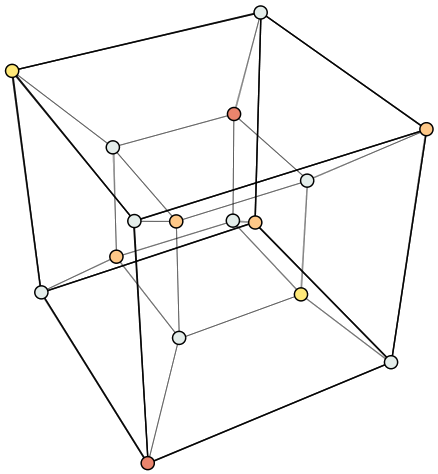
\includegraphics[scale=0.3]{pics/tesseract_fig1.png}}
	\column{0.5\textwidth}
	{\small
	\begin{itemize}
		\item Рассматриваемая нами модель имеет координаты $(x_1,x_2,x_3,x_4) \in R^4$, такие, что $x_1 \in [ -1,1 ]$. 
		\item Ограничивается восемью гиперплоскостями	
		\item Имеет 8 трехмерных граней, 24 двумерных, 32 ребра и 16 вершин.
	\end{itemize}
}
	\clearpage
\end{columns}
\end{frame}

\begin{frame}
\frametitle{Наглядный процесс формирования отображения тессеракта на трехмерную плоскость}
\begin{center}
	\framebox{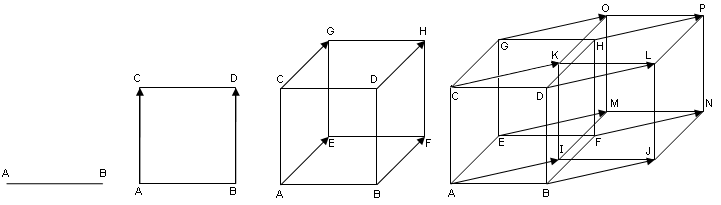
\includegraphics[scale=0.4]{pics/make_tess.png}} \\
\end{center}
Наглядный процесс, как точка $A$ переходит постепенно в гиперкуб, приобретая новые размерности
\end{frame}


\begin{frame}
	\frametitle{Графический пользовательский интерфейс}
	\begin{columns}
		\column{0.5\textwidth}
			\framebox{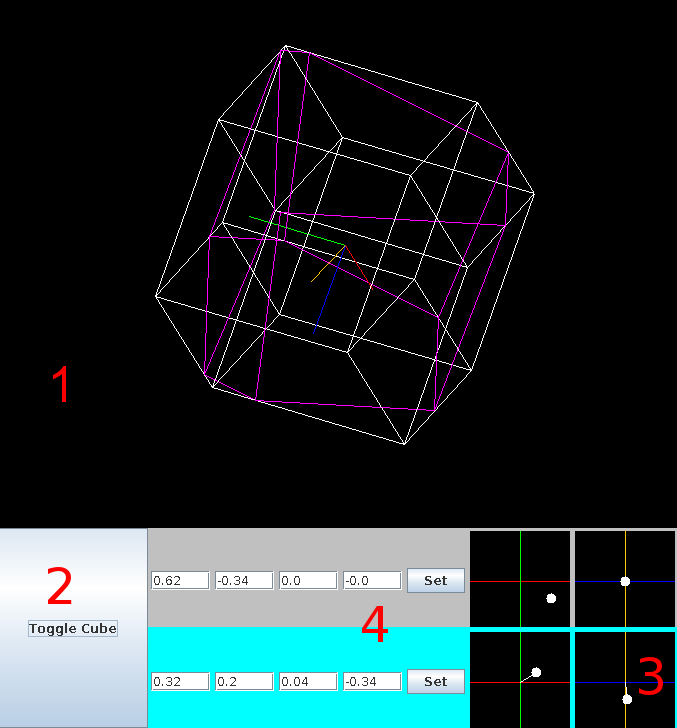
\includegraphics[scale=0.25]{pics/gui_numbers.png}}
		\column{0.5\textwidth}
			\begin{enumerate}
				\item Панель отображения
				\item Кнопка переключения отображения тессеракта
				\item Квадратные области графического ввода координат
				\item Панели ввода координат
			\end{enumerate}				
	\end{columns}
\end{frame}

\begin{frame}
\frametitle{Метод построения сечений тессеракта гиперплоскостью}
	\begin{itemize}
		\item Задание гиперплоскость сечения
		\item Нахождение точки пересечения гиперплоскости и тессеракта
		\item Поворот получившегося сечения до вложимости его в трехмерное пространство
		\item Вывод полученного сечения, анализ результатов
	\end{itemize}
\center{\framebox{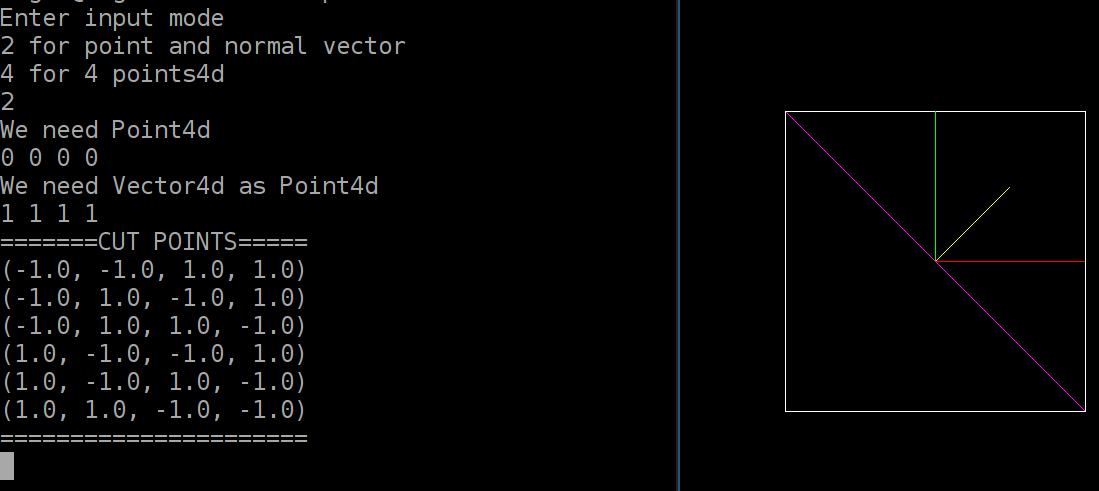
\includegraphics[scale=0.26]{pics/a1.png}}}
\end{frame}

\begin{frame}
\frametitle{История разработки: {\bf CubeCut3d}}
	top ayy	
	Сначала мы написали программу, которая 
	строит сечение обычного трёхмерного куба двухмерной плоскостью.
	Плоскость задавалась координатами трёх точек, которые задают плоскость сечения.
	Были реализованы механизмы поворота, масштабирования фигуры.	
	Не использовались никакие сторонние библиотеки для отображения графики,
	всё было написано с нуля. 
	\center{\framebox{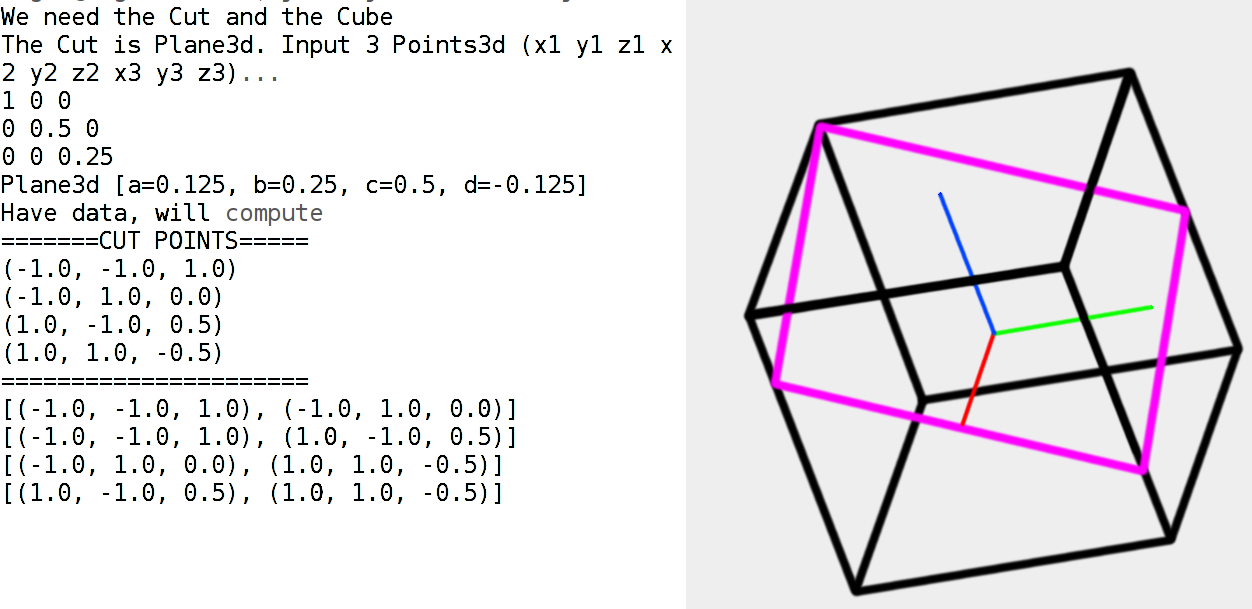
\includegraphics[scale=0.20]{pics/cubecut3d.png}}}
\end{frame}

\begin{frame}
\frametitle{История разработки: {\bf DrawTesseract}}
	Для перехода в четырёхмерное пространство нам нужно 
	было научиться строить изображения проекции тессеракта на двумерную плоскость.
	Так, основываясь на код первой версии, был написан код программы, которая строит
	проекцию гиперкуба и позваляет поворачивать изображение.
	\center{\framebox{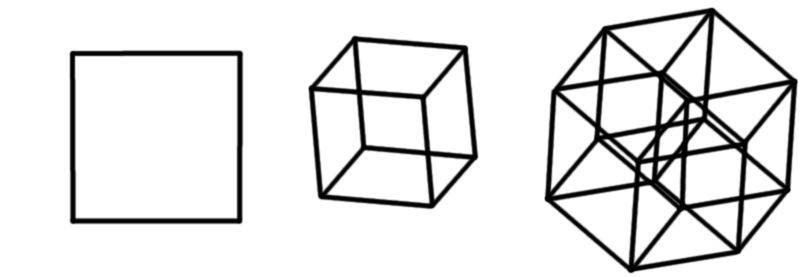
\includegraphics[scale=0.40]{pics/transformation.png}}} 
\end{frame}

\begin{frame}
\frametitle{История разработки: {\bf CutTesseract}}
	\begin{columns}
	\column{0.5\textwidth}
		Ипользуя принципы ООП (объектно-ориентированного программирования),
		было очень просто перейти из трёхмерного в четырёхмерный мир. 
		Плоскость всё ещё можно было задавать точками, только теперь нужно
		четыре четырёхмерных точек. Однако, задавать плоскость вектором нормали
		и точкой на плоскости оказалось удобнее с точки зрения ввода данных.
		Так и появились Квадратные области графического ввода координат.
	\column{0.5\textwidth}
		\center{\framebox{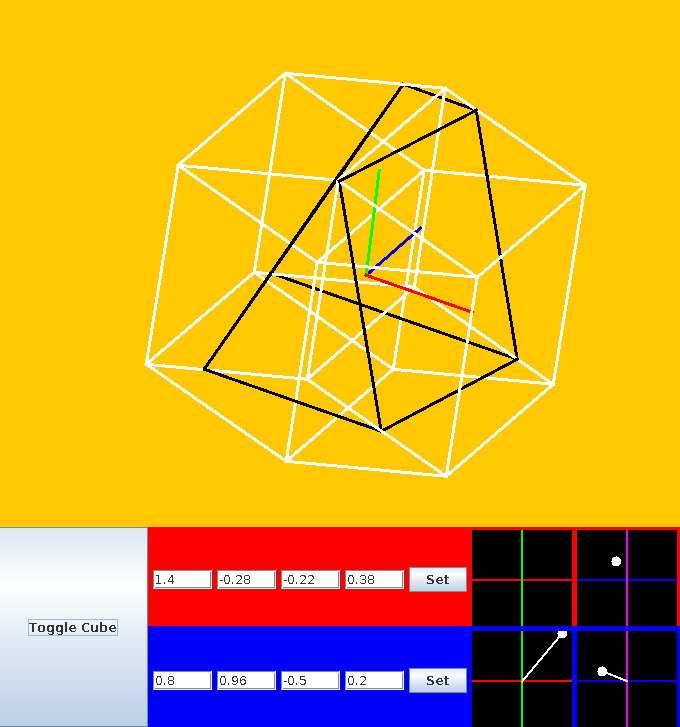
\includegraphics[scale=0.23]{pics/gui.png}}}
	\end{columns}
\end{frame}

\end{document}
